\section{Detection}

\begin{figure}[h!]
    \centering
        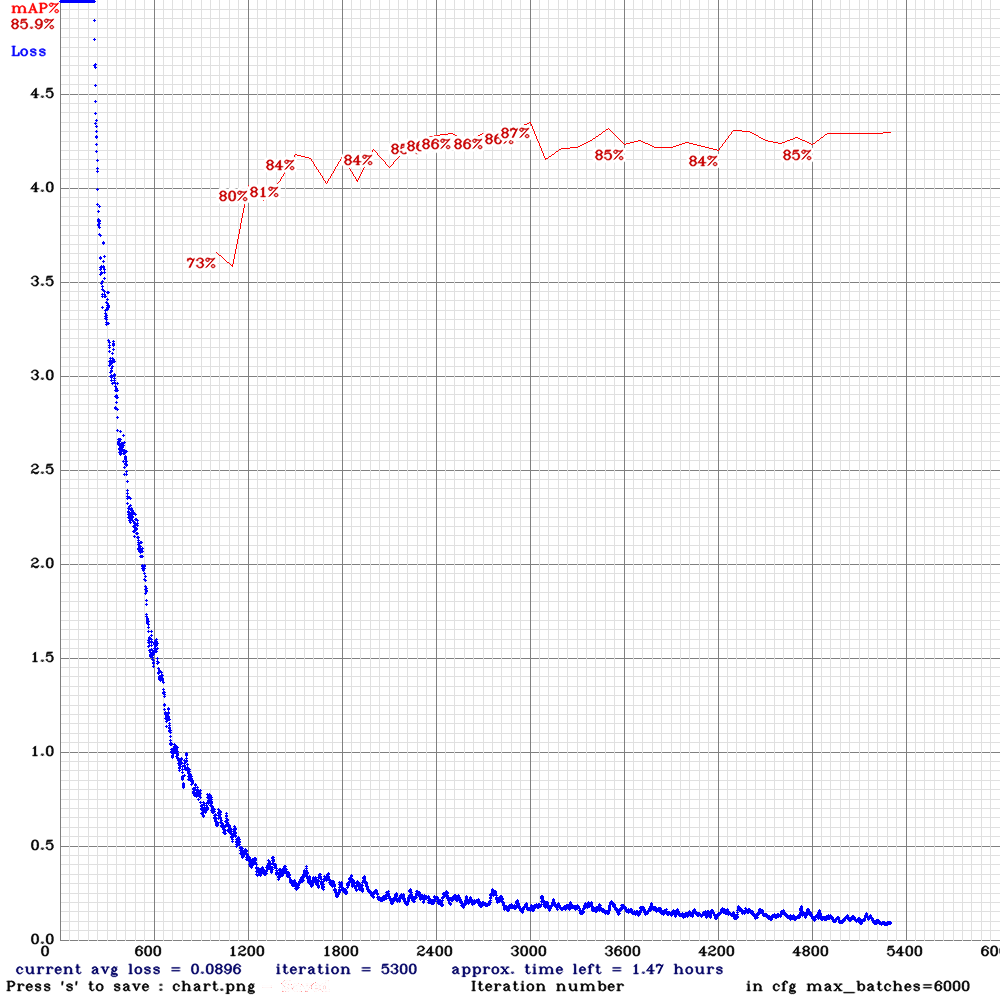
\includegraphics[width=0.4\textwidth]{pictures/painting_detection/training-v3.png}
    \caption{YOLOv3 trained on our custom dataset}
    \label{fig:training-v3}
\end{figure}



The detection of paintings and statues is done through a custom YOLOv3 neural network.\cite{yolov3}
Yolo is an architecture that provides a new approach to object detection, a single neural network predicts bounding boxes and class probabilities directly from full images in one evaluation.
In order to use this neural network we have labeled 1343 images, 805 of them have been used to train the network, 269 for the validation set and 269 for the test set, providing a total number of 3733 labels. The images of paintings and statues were taken by the frame extracted by some videos recorded in the Galleria Estense, for the person class was instead used a mix of labeled images taken from the previous videos and a some images of people in another museum.


The training has been performed with darknet \cite{darknet} taking the mAP every 1000 iterations \ref{fig:training-v3}, this allowed us to take the best weights that weren't affected by overfitting.
 %(AP=98.61\% for the class 'painting ', AP = 95.34\% for the class 'statue', AP = 34.08\% for the class 'person' and a final recall of 93.97\%).
In the end we got a powerful neural network with high performance and capable of a good generalization.

\begin{table*}[ht]
    \centering
    \begin{tabular}{|c|c|c|c|c|}
    \hline
    \multicolumn{5}{|c|}{\textbf{Detection   Performance}}  \\ \hline
    \multicolumn{1}{|l|}{} & \textbf{Painting} & \textbf{Statue} & \textbf{Person} & \textbf{Overall} \\ \hline
    \textbf{TP}        & 520     & 222     & 70      & 812  \\ \hline
    \textbf{FP}        & 133     & 18      & 28      & 179  \\ \hline
    \textbf{Precision} & 79.63\% & 92.50\% & 71.42\% & 82\% \\ \hline
    \textbf{Recall}    & -       & -       & -       & 85\% \\ \hline
    \textbf{IoU}       & -       & -       & -       & 70\% \\ \hline
    \end{tabular}
    \caption{Detection performance}
    \label{tab:detection_performance}
    \end{table*}

\begin{figure}[h]
    \centering
        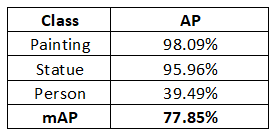
\includegraphics[width=0.4\textwidth]{pictures/painting_detection/tabella2.png}
    \caption{Average Precision and Mean Average Precision}
    %Histogram of Average Precision and Mean Average Precision
    \label{fig:figura3}
\end{figure}

\subsection{Comparison with previous technique}
In a previous pipeline the detection was made without neural networks:
the image was preprocessed and then we computed the edges with the Canny edge detector \cite{canny}. From the edges we took the signficant borders that identified the paintings and finally draw the region of interest around the borders. Despite this method worked well in the main scenery, it wasn't able to adapt to strong luminance variation and to manage the presence of shadows.
The accuracy that was produced didn't satisfy the standard of the project, for this reason we choose to implement a neural network.

